\documentclass[aspectratio=169,10pt]{beamer}

% Clean, minimal 16:9 presentation for a recorded LinkedIn video.
\usetheme{default}
\usepackage[T1]{fontenc}
\usepackage[utf8]{inputenc}
\usepackage{lmodern}
\usepackage{microtype}
\usepackage{xcolor}
\usepackage{tikz}
\usetikzlibrary{arrows.meta, positioning, calc}
\usepackage{listings}
\usepackage{hyperref}
\usepackage{booktabs}

\definecolor{DeepNavy}{HTML}{102A35}
\definecolor{Teal}{HTML}{167D83}
\definecolor{PaleTeal}{HTML}{E7F3F2}
\definecolor{Ink}{HTML}{24343B}
\definecolor{Muted}{HTML}{65757C}
\definecolor{CodeBg}{HTML}{F3F6F6}
\definecolor{CodeGreen}{HTML}{176B58}

\setbeamercolor{normal text}{fg=Ink,bg=white}
\setbeamercolor{structure}{fg=Teal}
\setbeamercolor{frametitle}{fg=DeepNavy,bg=white}
% Strong editorial slide-heading treatment: bold number, teal slash, bold title.
\setbeamerfont{frametitle}{size=\Large,series=\bfseries}
\newcommand{\slideheading}[2]{%
  {\fontfamily{phv}\fontseries{b}\selectfont\textcolor{DeepNavy}{#1}}%
  \hspace{0.16cm}{\fontfamily{phv}\fontseries{m}\selectfont\textcolor{Teal}{/}}%
  \hspace{0.16cm}{\fontfamily{phv}\fontseries{b}\selectfont\textcolor{DeepNavy}{#2}}%
}
\setbeamertemplate{frametitle}{%
  \vspace{0.12cm}%
  \nointerlineskip%
  \begin{beamercolorbox}[wd=\paperwidth,ht=3.6ex,dp=1.0ex,leftskip=8mm,rightskip=8mm]{frametitle}%
    \usebeamerfont{frametitle}\insertframetitle\strut
  \end{beamercolorbox}%
  \hspace*{8mm}\textcolor{Teal}{\rule{1.0cm}{2pt}}%
  \vspace{0.12cm}%
}
\setbeamercolor{title}{fg=white}
\setbeamercolor{subtitle}{fg=white!80}
\setbeamercolor{footline}{fg=Muted,bg=white}
\setbeamertemplate{navigation symbols}{}
\setbeamertemplate{footline}{%
  \leavevmode%
  \hbox{%
    \begin{beamercolorbox}[wd=.82\paperwidth,ht=2.7ex,dp=1.1ex,leftskip=1.1em]{footline}%
      \scriptsize WATER JUG PROBLEM SOLVER \hspace{0.5em} $\cdot$ \hspace{0.5em} GRAPH THEORY + BFS
    \end{beamercolorbox}%
    \begin{beamercolorbox}[wd=.18\paperwidth,ht=2.7ex,dp=1.1ex,rightskip=1.1em plus1fil]{footline}%
      \scriptsize \insertframenumber/\inserttotalframenumber
    \end{beamercolorbox}%
  }%
}
\setbeamersize{text margin left=8mm,text margin right=8mm}
\setlength{\parskip}{4pt}

\lstset{
  language=Python,
  basicstyle=\ttfamily\tiny,
  keywordstyle=\bfseries\color{Teal},
  commentstyle=\itshape\color{Muted},
  stringstyle=\color{CodeGreen},
  backgroundcolor=\color{CodeBg},
  frame=single,
  rulecolor=\color{CodeBg},
  frameround=ffff,
  framesep=5pt,
  xleftmargin=2pt,
  xrightmargin=2pt,
  showstringspaces=false,
  breaklines=true,
  columns=fullflexible,
  keepspaces=true,
  tabsize=4
}

\newcommand{\accentline}{\textcolor{Teal}{\rule{1.0cm}{2pt}}}
\newcommand{\smalllabel}[1]{\textcolor{Teal}{\bfseries\scriptsize #1}}
\newcommand{\jug}[2]{%
  \begin{tikzpicture}[baseline=(current bounding box.center)]
    \draw[DeepNavy,line width=1.1pt,rounded corners=2pt] (0,0) -- (0.08,0.95) -- (0.62,0.95) -- (0.70,0) -- cycle;
    \draw[Teal,line width=1pt] (0.06,{0.08+0.82*#1}) -- (0.64,{0.08+0.82*#1});
    \fill[Teal!18] (0.04,0.02) -- (0.66,0.02) -- (0.64,{0.08+0.82*#1}) -- (0.06,{0.08+0.82*#1}) -- cycle;
    \node[font=\scriptsize\bfseries,DeepNavy] at (0.35,-0.18) {#2};
  \end{tikzpicture}%
}

\begin{document}

% 1 — TITLE
{\setbeamertemplate{footline}{}
\begin{frame}[plain]
  \begin{tikzpicture}[remember picture,overlay]
    \fill[DeepNavy] (current page.south west) rectangle (current page.north east);
    \fill[Teal] (current page.south west) rectangle ([xshift=5mm]current page.north west);
    \draw[white,opacity=.12,line width=1pt] ([xshift=8.5cm,yshift=-1.2cm]current page.center) circle (2.8cm);
    \draw[white,opacity=.12,line width=1pt] ([xshift=8.5cm,yshift=-1.2cm]current page.center) circle (2.1cm);
    \draw[white,opacity=.12,line width=1pt] ([xshift=8.5cm,yshift=-1.2cm]current page.center) circle (1.4cm);
    \fill[Teal,opacity=.18] ([xshift=7.9cm,yshift=-2.5cm]current page.center) circle (1.15cm);
  \end{tikzpicture}
  \vspace{0.55cm}
  {\color{Teal}\bfseries\small GRAPH THEORY PROJECT}\par\vspace{0.35cm}
  {\usebeamerfont{title}\fontsize{29}{34}\selectfont\bfseries\color{white}Water Jug\par Problem Solver}\par
  \vspace{0.35cm}
  {\color{white!78}\large Finding a minimum-step solution with Breadth-First Search}\par
  \vspace{1.0cm}
  \accentline\par\vspace{0.35cm}
  {\color{white!72}\small A group project by}\par\vspace{0.12cm}
  {\color{white}\normalsize Glenda Pinhero \quad $\cdot$ \quad Gouri Krishna A}\par
  {\color{white}\normalsize Gayathri Jayan \quad $\cdot$ \quad Abhirami Mohan}
\end{frame}}

% 2 — PROBLEM AND RELEVANCE
\begin{frame}{\slideheading{01}{Understanding the problem}}
  \smalllabel{THE CHALLENGE}\par
  \vspace{0.15cm}
  \begin{columns}[T,onlytextwidth]
    \begin{column}{0.56\textwidth}
      {\LARGE\bfseries Can two fixed-capacity jugs\par measure an exact amount?}\par\vspace{0.25cm}
      The task is to obtain a target quantity of water using two jugs, without measurement markings.
      \vspace{0.25cm}
      \begin{itemize}
        \item Each jug has a fixed capacity.
        \item Water can be added, discarded, or transferred.
        \item The goal is to reach a state that contains the target amount.
      \end{itemize}
      \vspace{0.15cm}
      \textcolor{Muted}{\small Why it matters: a simple physical puzzle introduces search, planning, and algorithmic problem-solving.}
    \end{column}
    \begin{column}{0.40\textwidth}
      \begin{center}
        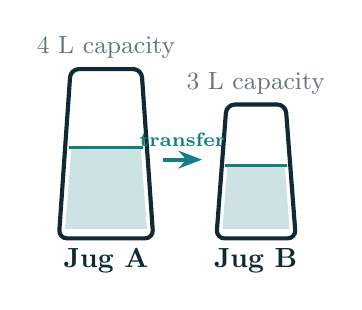
\begin{tikzpicture}[scale=1.0]
          \draw[DeepNavy,line width=1.5pt,rounded corners=3pt] (0,0) -- (0.15,2.15) -- (1.05,2.15) -- (1.20,0) -- cycle;
          \fill[Teal!22] (0.08,0.12) -- (1.12,0.12) -- (1.04,1.15) -- (0.16,1.15) -- cycle;
          \draw[Teal,line width=1.1pt] (0.13,1.15) -- (1.07,1.15);
          \node[DeepNavy,font=\bfseries] at (0.60,-0.28) {Jug A};
          \node[Muted,font=\small] at (0.60,2.42) {4 L capacity};
          \draw[DeepNavy,line width=1.5pt,rounded corners=3pt] (2.00,0) -- (2.13,1.70) -- (2.88,1.70) -- (3.01,0) -- cycle;
          \fill[Teal!22] (2.08,0.12) -- (2.93,0.12) -- (2.87,0.92) -- (2.14,0.92) -- cycle;
          \draw[Teal,line width=1.1pt] (2.11,0.92) -- (2.90,0.92);
          \node[DeepNavy,font=\bfseries] at (2.50,-0.28) {Jug B};
          \node[Muted,font=\small] at (2.50,1.97) {3 L capacity};
          \draw[-{Stealth[length=3mm]},Teal,line width=1.5pt] (1.32,1.00) -- (1.82,1.00);
          \node[Teal,font=\scriptsize\bfseries] at (1.57,1.25) {transfer};
        \end{tikzpicture}
        \vspace{0.3cm}
        \begin{beamercolorbox}[rounded=true,sep=8pt,wd=.92\linewidth]{normal text}
          \centering\color{DeepNavy}\bfseries Example goal\par
          \vspace{2pt}\normalfont\small Measure 2 litres using 4 L and 3 L jugs.
        \end{beamercolorbox}
      \end{center}
    \end{column}
  \end{columns}
\end{frame}

% 3 — OPERATIONS + STATE REPRESENTATION
\begin{frame}{\slideheading{02}{Permitted operations and state representation}}
  \begin{columns}[T,onlytextwidth]
    \begin{column}{0.49\textwidth}
      \smalllabel{PERMITTED OPERATIONS}\par\vspace{0.12cm}
      \begin{enumerate}
        \item \textbf{Fill} a jug to its capacity.
        \item \textbf{Empty} a jug completely.
        \item \textbf{Pour} from one jug into the other until the source is empty or the destination is full.
      \end{enumerate}
      \vspace{0.2cm}
      \begin{beamercolorbox}[rounded=true,sep=7pt,wd=\linewidth]{normal text}
        \color{Muted}\small Each operation changes the configuration, but never exceeds a jug's capacity.
      \end{beamercolorbox}
    \end{column}
    \begin{column}{0.47\textwidth}
      \smalllabel{STATE REPRESENTATION}\par\vspace{0.12cm}
      A state is an ordered pair:
      \[
        (a,b)
      \]
      \begin{itemize}
        \item $a$ = water currently in Jug A
        \item $b$ = water currently in Jug B
      \end{itemize}
      For capacities $C_A$ and $C_B$:
      \[
        0\leq a\leq C_A,\qquad 0\leq b\leq C_B
      \]
      \vspace{0.1cm}
      \begin{beamercolorbox}[rounded=true,sep=7pt,wd=\linewidth]{normal text}
        \centering\color{DeepNavy}\bfseries Start: $(0,0)$\qquad\bfseries Goal: $a=2$ or $b=2$
      \end{beamercolorbox}
    \end{column}
  \end{columns}
\end{frame}

% 4 — GRAPH MODEL
\begin{frame}{\slideheading{03}{Model it as a graph}}
  \begin{columns}[T,onlytextwidth]
    \begin{column}{0.46\textwidth}
      \smalllabel{STATE-SPACE MODEL}\par\vspace{0.12cm}
      \begin{itemize}
        \item Each node represents one valid state $(a,b)$.
        \item Each directed edge represents one permitted operation.
        \item The initial node is $(0,0)$.
        \item A goal node contains the target quantity.
      \end{itemize}
      \vspace{0.2cm}
      This turns the puzzle into a search problem: explore valid transitions until a goal state is found.
    \end{column}
    \begin{column}{0.52\textwidth}
      \centering
      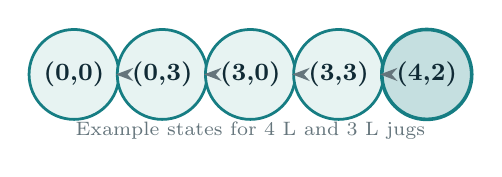
\begin{tikzpicture}[
        state/.style={circle,draw=Teal,line width=1pt,fill=PaleTeal,minimum size=8mm,font=\small\bfseries,text=DeepNavy},
        goal/.style={circle,draw=Teal,line width=1.3pt,fill=Teal!25,minimum size=8mm,font=\small\bfseries,text=DeepNavy},
        edge/.style={-{Stealth[length=2.2mm]},draw=Muted,line width=0.9pt}
      ]
        \node[state] (s0) at (0,0) {(0,0)};
        \node[state] (s1) at (1.12,0) {(0,3)};
        \node[state] (s2) at (2.24,0) {(3,0)};
        \node[state] (s3) at (3.36,0) {(3,3)};
        \node[goal] (s4) at (4.48,0) {(4,2)};
        \draw[edge] (s0) -- (s1);
        \draw[edge] (s1) -- (s2);
        \draw[edge] (s2) -- (s3);
        \draw[edge] (s3) -- (s4);
        \node[font=\scriptsize,text=Muted,align=center] at (2.24,-0.72) {Example states for 4 L and 3 L jugs};
      \end{tikzpicture}
      \vspace{0.25cm}
      {\scriptsize\color{Muted}The complete graph depends on the selected jug capacities.}
    \end{column}
  \end{columns}
\end{frame}

% 5 — BFS
\begin{frame}{\slideheading{04}{Why Breadth-First Search?}}
  \begin{columns}[T,onlytextwidth]
    \begin{column}{0.48\textwidth}
      \smalllabel{THE SEARCH STRATEGY}\par\vspace{0.12cm}
      BFS explores states in layers: first the start state, then all states one operation away, then two operations away, and so on.
      \vspace{0.2cm}
      \begin{enumerate}
        \item Add the start state to a FIFO queue.
        \item Remove the next state from the front.
        \item Generate valid next states.
        \item Record unseen states and continue until a goal is found.
      \end{enumerate}
    \end{column}
    \begin{column}{0.48\textwidth}
      \smalllabel{KEY DATA STRUCTURES}\par\vspace{0.12cm}
      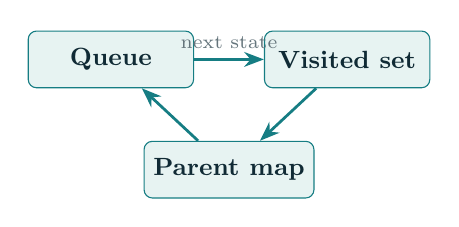
\begin{tikzpicture}[
        box/.style={rounded corners=3pt,draw=Teal,fill=PaleTeal,minimum width=2.1cm,minimum height=0.72cm,align=center,font=\small\bfseries,text=DeepNavy},
        arr/.style={-{Stealth[length=2.5mm]},line width=1pt,draw=Teal}
      ]
        \node[box] (q) at (0,1.15) {Queue};
        \node[box] (v) at (3.0,1.15) {Visited set};
        \node[box] (p) at (1.5,-0.25) {Parent map};
        \draw[arr] (q) -- node[above,font=\scriptsize,text=Muted]{next state} (v);
        \draw[arr] (v) -- (p);
        \draw[arr] (p) -- (q);
      \end{tikzpicture}
      \vspace{0.25cm}
      \begin{beamercolorbox}[rounded=true,sep=8pt,wd=\linewidth]{normal text}
        \textcolor{DeepNavy}{\bfseries Why BFS?}\par
        \small If every operation has equal cost, BFS finds a solution with the fewest operations.
      \end{beamercolorbox}
    \end{column}
  \end{columns}
\end{frame}

% 6 — STATE TRANSITIONS CODE
\begin{frame}[fragile]{\slideheading{05}{Implementation: valid jug operations}}
  \smalllabel{CORE LOGIC}\par\vspace{0.08cm}
  The solver applies the permitted operations to a state and produces its valid neighbours.
  \vspace{0.06cm}
  \begin{lstlisting}
def next_states(a, b, cap_a, cap_b):
    # Fill either jug
    yield (cap_a, b)
    yield (a, cap_b)

    # Empty either jug
    yield (0, b)
    yield (a, 0)

    # Pour A -> B
    move = min(a, cap_b - b)
    yield (a - move, b + move)

    # Pour B -> A
    move = min(b, cap_a - a)
    yield (a + move, b - move)
  \end{lstlisting}
  \vspace{0.1cm}
  {\scriptsize\color{Muted}Illustrative core logic: in a complete implementation, repeated states are filtered using a visited set. Function names can be aligned with the final project source.}
\end{frame}

% 7 — BFS CODE
\begin{frame}[fragile]{\slideheading{06}{Implementation: BFS solver}}
  \smalllabel{SEARCH + PATH TRACKING}\par\vspace{0.08cm}
  A queue drives the search; a parent map stores how each state was reached so the path can be reconstructed.
  \vspace{0.04cm}
  \begin{lstlisting}
from collections import deque

def bfs(start, is_goal, neighbours):
    queue = deque([start])
    parent = {start: None}

    while queue:
        state = queue.popleft()
        if is_goal(state):
            path = []
            while state is not None:
                path.append(state)
                state = parent[state]
            return path[::-1]

        for nxt in neighbours(state):
            if nxt not in parent:       # unseen state
                parent[nxt] = state
                queue.append(nxt)

    return None  # no solution found
  \end{lstlisting}
  \vspace{0.02cm}
  {\tiny\color{Muted}This is a compact, generic BFS illustration; the website demo will show the actual solver working on a chosen jug-capacity example.}
\end{frame}

% 8 — LIVE DEMO LINK (END SLIDE)
{\setbeamertemplate{footline}{}
\begin{frame}[plain]
  \begin{tikzpicture}[remember picture,overlay]
    \fill[DeepNavy] (current page.south west) rectangle (current page.north east);
    \fill[Teal] (current page.south west) rectangle ([xshift=5mm]current page.north west);
    \draw[white,opacity=.12,line width=1pt] ([xshift=7.7cm,yshift=-0.8cm]current page.center) circle (2.6cm);
    \draw[white,opacity=.12,line width=1pt] ([xshift=7.7cm,yshift=-0.8cm]current page.center) circle (1.8cm);
  \end{tikzpicture}
  \vspace{0.8cm}
  {\color{Teal}\bfseries\small TRY THE PROJECT}\par\vspace{0.35cm}
  {\fontsize{27}{32}\selectfont\bfseries\color{white}Explore the Water Jug\par Solver}\par\vspace{0.35cm}
  {\color{white!75}\large Watch the states change as BFS finds a solution.}\par\vspace{0.8cm}
  \begin{beamercolorbox}[rounded=true,sep=12pt,wd=.88\linewidth]{normal text}
    {\color{Muted}\scriptsize LIVE DEMO WEBSITE}\par\vspace{0.12cm}
    {\large\bfseries\href{https://water-jug-solver-zgcfjkasx5rqv2nsggwbnf.streamlit.app/}{\textcolor{Teal}{water-jug-solver.streamlit.app}}}\par\vspace{0.08cm}
    {\scriptsize\url{https://water-jug-solver-zgcfjkasx5rqv2nsggwbnf.streamlit.app/}}
  \end{beamercolorbox}
  \vspace{0.75cm}
  {\color{white!72}\small Glenda Pinhero \quad $\cdot$ \quad Gouri Krishna A \quad $\cdot$ \quad Gayathri Jayan \quad $\cdot$ \quad Abhirami Mohan}
\end{frame}}

\end{document}
